\documentclass[11pt,a4paper]{article}
\usepackage[T1]{fontenc}
\usepackage[utf8]{inputenc}
\usepackage{amsmath,amsthm,mathtools}
\usepackage{newpxtext,newpxmath}
\usepackage[margin=27mm,headheight=15pt]{geometry}
\usepackage{microtype}
\usepackage{booktabs,array,longtable}
\usepackage{graphicx}
\usepackage{tikz}
\usetikzlibrary{arrows.meta,positioning,automata}
\usepackage[dvipsnames]{xcolor}
\definecolor{ink}{HTML}{28352B}
\definecolor{accent}{HTML}{536B46}
\usepackage{hyperref}
\hypersetup{colorlinks=true,linkcolor=accent,citecolor=accent,urlcolor=accent,
 pdftitle={Mutual-visibility sets in Andrasfai graphs},
 pdfauthor={ChatGPT; prepared for Vladimir Reshetnikov},
 pdfsubject={A proof of the generating-function conjecture in OEIS A391632}}
\usepackage[nameinlink,noabbrev]{cleveref}
\usepackage{fancyhdr}
\pagestyle{fancy}
\fancyhf{}
\fancyhead[L]{\small Andr\'asfai mutual visibility}
\fancyhead[R]{\small A391632}
\fancyfoot[C]{\thepage}
\renewcommand{\headrulewidth}{0.3pt}
\usepackage{enumitem}
\setlist{itemsep=3pt,topsep=5pt}
\newtheorem{theorem}{Theorem}[section]
\newtheorem{lemma}[theorem]{Lemma}
\newtheorem{proposition}[theorem]{Proposition}
\newtheorem{corollary}[theorem]{Corollary}
\theoremstyle{definition}
\newtheorem{definition}[theorem]{Definition}
\newtheorem{remark}[theorem]{Remark}
\newcommand{\Z}{\mathbb Z}
\newcommand{\R}{\mathbb R}
\newcommand{\Q}{\mathbb Q}
\newcommand{\E}{\mathbb E}
\newcommand{\Var}{\operatorname{Var}}
\newcommand{\tr}{\operatorname{tr}}
\newcommand{\MV}{\mathcal M}
\newcommand{\V}{\mathcal V}
\newcommand{\bits}{\{0,1\}}
\newcommand{\Andr}{\operatorname{And}}
\newcommand{\eps}{\varepsilon}
\newcommand{\Ngraph}{\Gamma}
\allowdisplaybreaks[2]
\setlength{\parindent}{1.25em}
\setlength{\parskip}{3pt}
\emergencystretch=1.5em

\title{\vspace{-1.3cm}\color{ink}\bfseries Mutual-visibility sets in Andr\'asfai graphs\par
\large A four-state proof of OEIS A391632, with cardinality refinements}
\author{ChatGPT\\\small Research report prepared for Vladimir Reshetnikov}
\date{19 September 2026}

\begin{document}
\maketitle
\thispagestyle{empty}
\begin{abstract}
We prove the rational generating function conjectured by Andrew Howroyd in
OEIS A391632 for the number of mutual-visibility sets in Andr\'asfai graphs.
The proof translates the common-neighbor obstruction into an infinite family
of forbidden cyclic binary patterns, then recognizes that family with a
four-state weighted automaton. A uniqueness argument for periodic auxiliary
flags is essential: it makes the trace of a matrix power count each labeled
vertex subset exactly once. Keeping a variable for cardinality gives the full
bivariate generating function. We also obtain an explicit binomial formula,
classify the maximum sets, prove eventual polynomiality at every fixed deficit
from maximum size, derive exponential growth and a central limit theorem,
and give exact recognition and sampling algorithms. Independent exhaustive
checks cover all 9,586,980 subsets of the first eight graphs; symbolic checks
verify the displayed algebra. The proof is self-contained and does not depend
on those finite checks.
\end{abstract}

\noindent\textbf{Status and scope.}
The OEIS entry, consulted on 19 September 2026, still labels the generating
function as conjectured \cite{oeis}. The argument here establishes that
statement and the refinements below. Targeted literature searches did not
identify an earlier proof, but they do not certify global priority. This
report has not been independently refereed or formalized in a proof
assistant. The executable checks and all source files accompany the report.

\vspace{6pt}
\noindent\textbf{Keywords.}
Mutual visibility; Andr\'asfai graph; cyclic word; finite automaton;
transfer matrix; rational generating function; fixed-deficit enumeration.

\vspace{10pt}
\noindent\textbf{Main identity.}
For the size-enumerator $V_n(y)$ of the $n$th graph,
\[
 V_n(y)=\tr\!\left(
 \begin{pmatrix}
 1&y&0&0\\1&0&y&0\\0&0&0&1\\0&1+y&0&0
 \end{pmatrix}^{\!3n-1}\right)\qquad(n\ge2).
\]
The exceptional graph $\Andr(1)=K_2$ has $V_1(y)=(1+y)^2$.

\clearpage
\tableofcontents
\clearpage

\section{The conjecture and the enumeration problem}
\label{sec:problem}

A set $S$ of vertices of a graph is a \emph{mutual-visibility set} when every
pair of distinct vertices of $S$ can be joined by a shortest path whose
internal vertices lie outside $S$. The condition is existential: one suitable
shortest path is enough. It does not require every shortest path to avoid
$S$. We use the definition introduced by Di Stefano \cite{distefano}.
In particular, the empty set, every singleton, and every two-element set
are mutual-visibility sets in any connected graph.

We use the standard circulant realization of the Andr\'asfai graph
\cite{metric}. For an integer $n\ge1$, put
\begin{equation}
 N=3n-1,\qquad
 G_n=\Andr(n)=\operatorname{Cay}\bigl(\Z/N\Z,\{1,4,7,\ldots,3n-2\}\bigr).
 \label{eq:graph}
\end{equation}
All vertex indices below are taken modulo $N$. The connection set is closed
under negation, since $N\equiv2\pmod3$; thus the graph is undirected. Each
vertex has $n$ neighbors. Our count is on this fixed labeled vertex set:
rotations and other graph automorphisms do \emph{not} identify subsets.

Write
\begin{equation}
 \MV_n=\{S\subseteq\Z/N\Z:S\text{ is a mutual-visibility set of }G_n\},
 \qquad
 V_n(y)=\sum_{S\in\MV_n}y^{|S|},\qquad a_n=V_n(1).
 \label{eq:enumerator}
\end{equation}
The variable $y$ marks the cardinality of the set; $x$ will mark the graph
index $n$. This distinction matters because the number of vertices is
$3n-1$, not $n$.

OEIS A391632 records $a_n$, beginning
\[
4,\ 21,\ 127,\ 749,\ 4455,\ 26725,\ 161007,\ 971613,\ldots.
\]
The entry was created by Eric W. Weisstein on 14 December 2025. On
12 January 2026, Andrew Howroyd supplied the following conjecture
\cite{oeis}:
\begin{equation}
 \sum_{n\ge1}a_nx^n=
 \frac{x(4-19x+33x^2-40x^3+8x^4)}
 {1-10x+29x^2-32x^3+8x^4}.
 \label{eq:conjecture}
\end{equation}
The goal is to explain this identity combinatorially, not simply to extend
the sequence or fit its recurrence.

\begin{theorem}[Counting theorem]
\label{thm:main}
Let
\begin{equation}
 M(y)=\begin{pmatrix}
 1&y&0&0\\
 1&0&y&0\\
 0&0&0&1\\
 0&1+y&0&0
 \end{pmatrix}.
 \label{eq:M}
\end{equation}
Then, for every $n\ge1$,
\begin{equation}
 V_n(y)=\tr M(y)^{3n-1}+\boldsymbol{1}_{\{n=1\}}y^2.
 \label{eq:maintrace}
\end{equation}
Consequently, \cref{eq:conjecture} holds.
\end{theorem}

The proof occupies \cref{sec:patterns,sec:automaton,sec:gf}. Its difficult
point is not matrix inversion. It is proving that a cyclic word corresponds
to exactly one closed automaton walk; an arbitrary deterministic automaton
for linear words would not by itself justify a trace formula.

\section{From shortest paths to forbidden cyclic patterns}
\label{sec:patterns}

\subsection{The common-neighbor interval}

Let $\Ngraph(v)$ denote the neighborhood of a vertex $v$ in $G_n$.

\begin{lemma}
\label{lem:neighbors}
For $n\ge2$, every unordered nonadjacent pair has a unique orientation
$(a,a+3r-1)$ with $1\le r\le n-1$. Its common neighbors are exactly
\begin{equation}
 \Ngraph(a)\cap\Ngraph(a+3r-1)
   =\{a+1,a+4,\ldots,a+3r-2\}.
 \label{eq:common}
\end{equation}
In particular, $G_n$ has diameter two.
\end{lemma}

\begin{proof}
For a nonedge, the two positive oriented differences sum to $N$ and neither
is congruent to $1$ modulo $3$. Since $N\equiv2\pmod3$, one difference is
congruent to $0$ and the other to $2$. The latter is uniquely $3r-1$ with
$1\le r\le n-1$.

By translation, take $a=0$ and write $b=3r-1$. A neighbor of $0$ is a vertex
$v=1+3j$, with $0\le j\le n-1$. If $j\le r-1$, then $v<b$ and
\[
 b-v=3(r-j)-2\equiv1\pmod3,
\]
so $v$ is adjacent to $b$. If $j\ge r$, then $v>b$ and
$v-b\equiv2\pmod3$, so it is not adjacent to $b$. This proves the displayed
intersection. It is nonempty, so each nonedge has distance two; nonedges
exist for $n\ge2$.
\end{proof}

Adjacent selected vertices are always visible to one another using their
edge. For a nonadjacent pair, a shortest path has one internal vertex, and
that vertex must be a common neighbor. Therefore visibility fails precisely
when the endpoints and \emph{all} their common neighbors belong to $S$.

\subsection{Membership words and the infinite forbidden family}

Encode $S$ by its periodic membership word $(w_t)_{t\in\Z}$, with period $N$,
where $w_t=1$ exactly when $t\bmod N\in S$. By \cref{lem:neighbors}, $S$ fails
to be mutually visible precisely when there are $a$ and $r$, with
$1\le r\le n-1$, such that
\begin{equation}
 w_a=w_{a+3r-1}=w_{a+1}=w_{a+4}=\cdots=w_{a+3r-2}=1.
 \label{eq:obstruction}
\end{equation}
If a star denotes an arbitrary binary symbol, this is the pattern
\begin{equation}
 \mathcal F_r=11(\ast\ast1)^{r-1}1.
 \label{eq:forbidden}
\end{equation}
For example, the first three patterns are
$111$, $11\ast\ast11$, and $11\ast\ast1\ast\ast11$.
The stars are independent: they impose no requirement of being zero.

The original graph only supplies the range $r\le n-1$. For a uniform
finite-state description, we need to remove that bound without introducing
new restrictions.

\begin{lemma}[Periodic extension]
\label{lem:extension}
For $n\ge2$, a period-$N$ word avoids $\mathcal F_r$ for
$1\le r\le n-1$ if and only if it avoids $\mathcal F_r$ for every $r\ge1$.
\end{lemma}

\begin{proof}
Only the forward direction needs proof. Suppose an occurrence of
$\mathcal F_r$ begins at $a$ with $r\ge n$. Among its mandatory ones are
$w_a$, $w_{a+1}$, and $w_{a+3n-2}$. Since $3n-2=N-1$, the last of these
is $w_{a-1}$ by periodicity. Thus $w_{a-1}w_aw_{a+1}=111$, an occurrence
of $\mathcal F_1$. Since $n\ge2$, that pattern was already forbidden.
\end{proof}

It is important that the first graph is excluded here. For $n=1$, $G_1=K_2$
has no nonedges and all four subsets are valid. Repeating its full-set word
$11$ nevertheless produces $111$. This is the source of the correction
term in \cref{eq:maintrace}, and later of the precise starting index of the
scalar recurrence.

\section{A four-state automaton, with a cyclic uniqueness proof}
\label{sec:automaton}

\subsection{Auxiliary flags retain arbitrarily long prefixes}

For a binary word indexed by all integers, let $b_t$ be true if a finite
pattern of the form
\begin{equation}
 11(\ast\ast1)^{r-1},\qquad r\ge1,
 \label{eq:prefix}
\end{equation}
ends at position $t$. This is the forbidden pattern with its final $1$
removed. The flag asks whether reading another $1$ next would complete an
obstruction.

Using Boolean multiplication for conjunction, its recurrence is
\begin{equation}
 b_t=w_t\bigl(w_{t-1}\lor b_{t-3}\bigr).
 \label{eq:flag}
\end{equation}
Indeed, either the prefix is the initial $11$, or an earlier such prefix
ends three positions before $t$ and is extended by two arbitrary bits and
a final $1$. The word avoids all forbidden patterns if and only if
\begin{equation}
 b_t w_{t+1}=0\qquad\text{for every }t.
 \label{eq:reject}
\end{equation}

An apparent problem remains: a recurrence on a circle can have several
solutions, or a solution supported by a circular chain with no finite
starting witness. The arithmetic of $N$ rules this out.

\begin{lemma}[Uniqueness of periodic flags]
\label{lem:unique}
Let $N=3n-1$ and let a period-$N$ binary word contain a zero. There is exactly
one period-$N$ Boolean solution of \cref{eq:flag}. That solution has the
finite-prefix interpretation \cref{eq:prefix}.
\end{lemma}

\begin{proof}
Choose $z$ with $w_z=0$. Necessarily $b_z=0$. Since
$\gcd(3,N)=1$, the residues
\[
 z,\ z+3,\ z+6,\ldots,z+3(N-1)
\]
run through all vertices. Starting with $b_z=0$, recurrence
\cref{eq:flag} determines the flag at each subsequent residue from the
previous one. On returning to $z$, the equation still reads $b_z=0$
regardless of the incoming flag. Thus a unique periodic solution exists.

The flags defined by finite occurrences of \cref{eq:prefix} are periodic and
satisfy the same recurrence: a witnessed prefix either has length two or
has a shorter witnessed prefix three positions earlier. Conversely, both
terms on the right of \cref{eq:flag} create a finite witness. Hence those
semantic flags form a solution, and uniqueness identifies it with the one
just constructed. Equivalently, backwards substitution by steps of three
must encounter a zero, preventing an unsupported circular chain.
\end{proof}

The all-ones word is never accepted: \cref{eq:flag} forces all flags to one,
which violates \cref{eq:reject}. Consequently, the uniqueness lemma applies
to every accepted word.

\subsection{Six semantic states}

Consider the state immediately after reading position $t$:
\[
 (w_t,b_t,b_{t-1},b_{t-2}).
\]
Under \cref{eq:flag,eq:reject}, no two of $b_t,b_{t-1},b_{t-2}$ can be one.
Adjacent flags are impossible because $b_{t-1}=1$ forces $w_t=0$, whereas
$b_t=1$ forces $w_t=1$. If $b_t=b_{t-2}=1$, then $w_{t-1}=0$ by
\cref{eq:reject}; \cref{eq:flag} then forces $b_{t-3}=1$, contradicting
the impossibility of the adjacent pair $b_{t-3}=b_{t-2}=1$.

The only possible states and their transitions are therefore the following.
A dash means rejection. Edge labels are the bit being read, not a state
weight.
\begin{center}
\begin{tabular}{@{}clcc@{}}
\toprule
State & $(w_t,b_t,b_{t-1},b_{t-2})$ & Read $0$ & Read $1$\\
\midrule
$A$   & $(0,0,0,0)$ & $A$ & $B_1$\\
$B_1$ & $(1,0,0,0)$ & $A$ & $C$\\
$C$   & $(1,1,0,0)$ & $D$ & ---\\
$D$   & $(0,0,1,0)$ & $B_2$ & $B_3$\\
$B_2$ & $(0,0,0,1)$ & $A$ & $C$\\
$B_3$ & $(1,0,0,1)$ & $A$ & $C$\\
\bottomrule
\end{tabular}
\end{center}

To check the table mechanically, from $(a,b,c,d)$ a new bit $\eps$ is
forbidden when $b\eps=1$. Otherwise the new state is
\begin{equation}
 (a,b,c,d)\longmapsto
 \bigl(\eps,\eps(a\lor d),b,c\bigr).
 \label{eq:sixtransition}
\end{equation}
Thus the table is an exact local restatement of the flag recurrence and the
rejection rule, not a guessed automaton.

\subsection{Merging states without changing cyclic multiplicities}

The three states $B_1,B_2,B_3$ have identical outgoing labeled transitions.
Merge them to a single state $B$. The four-state labeled graph is shown in
\cref{fig:automaton}.

\begin{figure}[htbp]
\centering
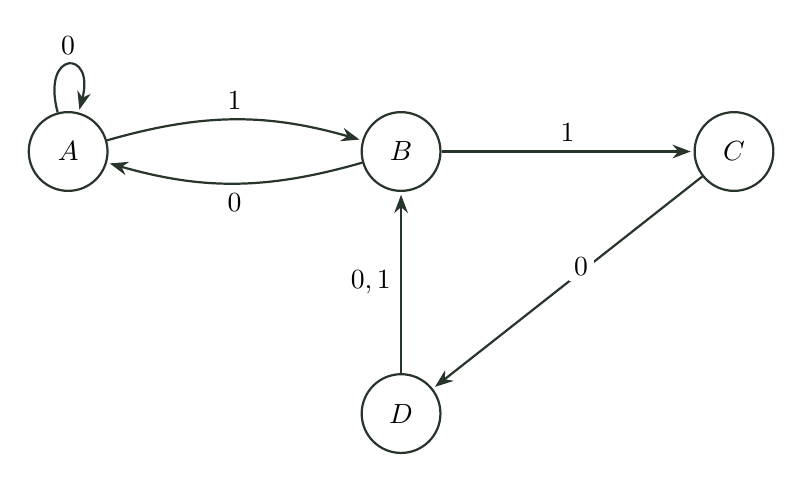
\begin{tikzpicture}[>=Stealth,shorten >=1pt,node distance=32mm,
 every state/.style={minimum size=10mm,draw=ink,thick},
 every edge/.style={draw=ink,thick},every node/.style={font=\normalsize}]
\node[state] (A) {$A$};
\node[state,right=of A] (B) {$B$};
\node[state,right=of B] (C) {$C$};
\node[state,below=23mm of B] (D) {$D$};
\path[->]
 (A) edge[loop above] node {$0$} (A)
 (A) edge[bend left=16] node[above] {$1$} (B)
 (B) edge[bend left=16] node[below] {$0$} (A)
 (B) edge node[above] {$1$} (C)
 (C) edge node[above right,fill=white,inner sep=2pt] {$0$} (D)
 (D) edge node[left] {$0,1$} (B);
\end{tikzpicture}
\caption{The four-state labeled automaton. The $D\to B$ arrow denotes two
 distinct edges, with labels $0$ and $1$. Weighting a label $1$ by $y$ and a
 label $0$ by $1$ gives the matrix $M(y)$.}
\label{fig:automaton}
\end{figure}

A quotient of a state graph need not preserve the number of closed walks.
Here it does, for an explicit reason. Each incoming edge to $B$ determines
the original state uniquely:
\begin{equation}
 A\xrightarrow{1}B\ \leadsto\ B_1,\qquad
 D\xrightarrow{0}B\ \leadsto\ B_2,\qquad
 D\xrightarrow{1}B\ \leadsto\ B_3.
 \label{eq:lift}
\end{equation}
There are no other incoming edges to $B$. The other states lift identically.
Every labeled closed walk in the quotient therefore lifts to exactly one
labeled closed walk in the six-state graph, and conversely.

\begin{proposition}[Anchored cyclic bijection]
\label{prop:bijection}
For $n\ge2$, the mutual-visibility sets of $G_n$ are in weight-preserving
bijection with the length-$N$ closed labeled walks in the four-state graph,
with a fixed time origin. The weight of a walk is $y$ to the number of its
edges labeled $1$.
\end{proposition}

\begin{proof}
Given a valid membership word $w_0,\ldots,w_{N-1}$, extend it periodically.
By \cref{lem:extension}, it avoids every forbidden pattern. Its unique
semantic flags produce a periodic six-state walk, and quotienting gives a
closed four-state walk. Start immediately before reading vertex $0$, so
there is no choice of a rotation or of a distinguished vertex.

Conversely, a closed four-state labeled walk lifts uniquely by
\cref{eq:lift}. Its sequence of emitted bits is periodic, and the lifted
states satisfy \cref{eq:flag,eq:reject}. The word cannot be all ones, so
\cref{lem:unique} identifies these flags with the semantic flags. Hence
all forbidden patterns are absent. By \cref{lem:neighbors,lem:extension},
the corresponding subset is mutually visible.

These constructions are inverse: the membership word fixes the semantic
flags, then all six states, and hence the four states. Each selected vertex
emits exactly one label $1$, so weights are preserved.
\end{proof}

The $(i,i)$ entry of $M(y)^N$ enumerates the closed walks with initial state
$i$. Summing over initial states gives the trace. This proves
\cref{eq:maintrace} for $n\ge2$. For $n=1$,
$\tr M(y)^2=1+2y$, while $V_1(y)=1+2y+y^2$, proving the remaining case.

\begin{remark}[Why there is no factor $1/N$]
A subset is a word on fixed vertices, not a necklace. Its state at the
boundary before vertex $0$ is forced. Trace sums the possible states at that
fixed boundary; it does not freely choose a boundary along the word.
Dividing the trace by $N$ would therefore be incorrect. Even periodic words
have one anchored state sequence, not several copies arising from a
symmetry.
\end{remark}

\section{Generating functions and recurrences}
\label{sec:gf}

\subsection{The full cardinality generating function}

The characteristic polynomial of $M(y)$ is
\begin{equation}
 F(z,y)=z^4-z^3-yz^2-y(1+y)z+y(1+y).
 \label{eq:char}
\end{equation}
Define $\V(x,y)=\sum_{n\ge1}V_n(y)x^n$. From the trace theorem and a formal
matrix geometric series,
\begin{align}
 \V(x,y)
 &=y^2x+x\,\tr\!\left(M(y)^2\sum_{j\ge0}x^jM(y)^{3j}\right)\notag\\
 &=y^2x+x\,\tr\!\left(M(y)^2(I-xM(y)^3)^{-1}\right).
 \label{eq:resolvent}
\end{align}
The inverse exists as a formal power series because its matrix argument has
constant term $I$.

\begin{theorem}[Bivariate rational form]
\label{thm:bivariate}
The generating function is $\V(x,y)=P(x,y)/D(x,y)$, where
\begin{align}
D(x,y)={}&1-(3y^2+6y+1)x\notag\\
 &+y(3y^3+11y^2+12y+3)x^2\notag\\
 &-y^2(y+1)^3(y+3)x^3+y^3(y+1)^3x^4,
 \label{eq:D}\\[3pt]
P(x,y)={}&(1+y)^2x-y(3y^3+7y^2+6y+3)x^2\notag\\
 &+y^2(3y^4+10y^3+11y^2+6y+3)x^3\notag\\
 &-y^3(y+1)^3(y^2+3y+1)x^4+y^5(y+1)^3x^5.
 \label{eq:P}
\end{align}
\end{theorem}

\begin{proof}
Starting from \cref{eq:resolvent}, multiply by
$D=\det(I-xM^3)$ and use the adjugate formula. Direct expansion gives
\cref{eq:D} and
\[
 P=y^2xD+x\,\tr\bigl(M^2\operatorname{adj}(I-xM^3)\bigr),
\]
whose expansion is \cref{eq:P}. These are finite polynomial identities,
independently checked by the supplied symbolic certificate.
\end{proof}

Putting $y=1$ in \cref{eq:D,eq:P} yields precisely
\cref{eq:conjecture}, completing the proof of \cref{thm:main}.
As a basic check on cardinality marking, at $y=0$ the rational expression
reduces to $x/(1-x)$: there is one empty set for each graph.

\subsection{The recurrence and its initial exception}

\begin{corollary}
\label{cor:recurrence}
The sequence $a_n$ satisfies
\begin{equation}
 a_n=10a_{n-1}-29a_{n-2}+32a_{n-3}-8a_{n-4}
 \qquad(n\ge6),
 \label{eq:recurrence}
\end{equation}
with initial values
\[
 a_1=4,\quad a_2=21,\quad a_3=127,\quad a_4=749,\quad a_5=4455.
\]
The eventual recurrence has minimal order four over $\Q$.
\end{corollary}

\begin{proof}
Compare coefficients in \cref{eq:conjecture}. The numerator has degree five,
so the homogeneous relation begins at $n=6$. The numerator and denominator
are coprime over $\Q$; the reduced denominator has degree four, which is
the minimum order of any eventual constant-coefficient recurrence.
\end{proof}

Starting \cref{eq:recurrence} at $n=5$ would give $4447$, not $4455$.
The residual is $8$, exactly the coefficient of $x^5$ in the numerator.
Alternatively set $c_1=3$ and $c_n=a_n$ for $n\ge2$. Then
$c_n=\tr M(1)^{3n-1}$ satisfies the same homogeneous recurrence for $n\ge5$.
The change at $n=1$ accounts for all of the discrepancy.

The coefficient polynomials themselves satisfy, for $n\ge6$,
\begin{align}
 V_n={}&(3y^2+6y+1)V_{n-1}
 -y(3y^3+11y^2+12y+3)V_{n-2}\notag\\
 &+y^2(y+1)^3(y+3)V_{n-3}-y^3(y+1)^3V_{n-4}.
 \label{eq:polyrec}
\end{align}
The first polynomials are
\begin{align*}
V_1={}&1+2y+y^2,\\
V_2={}&1+5y+10y^2+5y^3,\\
V_3={}&1+8y+28y^2+48y^3+34y^4+8y^5,\\
V_4={}&1+11y+55y^2+154y^3+242y^4+198y^5+77y^6+11y^7,\\
V_5={}&1+14y+91y^2+350y^3+847y^4+1274y^5\notag\\
 &+1141y^6+576y^7+147y^8+14y^9.
\end{align*}
The coefficients of $1,y,y^2$ are $1,N,\binom N2$, as required directly by
the definition. The appendix records further scalar values, while the
archive supplies the entire coefficient triangle through $n=50$.

\section{Return blocks and a finite binomial formula}
\label{sec:blocks}

\subsection{First returns to the state \texorpdfstring{$B$}{B}}

The automaton has only two types of first-return walk from $B$ to $B$:
\begin{equation}
 B\xrightarrow{0}A\xrightarrow{0}\cdots\xrightarrow{0}A
 \xrightarrow{1}B,
 \qquad
 B\xrightarrow{1}C\xrightarrow{0}D\xrightarrow{\eps}B,
 \quad\eps\in\bits.
 \label{eq:blocks}
\end{equation}
The first type has $j\ge0$ self-loops at $A$, length $j+2$, and weight $y$.
The second has length three and weights $y$ and $y^2$. Thus, if $z$ marks
walk length, the first-return series is
\begin{equation}
 H(z,y)=\frac{yz^2}{1-z}+y(1+y)z^3.
 \label{eq:H}
\end{equation}

Every closed walk other than the all-$A$ loop visits $B$. A walk that never
visits $A$ consists entirely of $B,C,D$ rounds and has length divisible by
three. Our lengths $N=3n-1$ are not divisible by three, so every nonzero
membership word under consideration has at least one first-type block.

There is a useful scalar determinant identity:
\begin{equation}
 \det(I-zM(y))=(1-z)(1-H(z,y)).
 \label{eq:detH}
\end{equation}
For example, expansion of the right side gives
$1-z-yz^2-y(1+y)z^3+y(1+y)z^4$, the reciprocal characteristic
polynomial from \cref{eq:char}.

If $T_N(y)=\tr M(y)^N$, logarithmic differentiation gives the formal identity
\begin{equation}
 \sum_{N\ge1}T_N(y)z^N
 =-z\frac{d}{dz}\log\det(I-zM(y))
 =\frac{z}{1-z}+\frac{zH_z(z,y)}{1-H(z,y)}.
 \label{eq:traceH}
\end{equation}
One can verify the first equality without any spectral assumptions:
Jacobi's determinant formula gives
$z\tr((I-zM)^{-1}M)=\sum_{N\ge1}\tr(M^N)z^N$.

Expanding $-\log(1-H)$ in \cref{eq:traceH} yields
\begin{equation}
 T_N(y)=1+N[z^N]\sum_{r\ge1}\frac{H(z,y)^r}{r}.
 \label{eq:logsum}
\end{equation}
This identity automatically handles periodic arrangements of blocks. In
particular, the denominator $r$ is not an unsupported division of a necklace
count by its length.

\subsection{An explicit count of every cardinality}

\begin{theorem}[Binomial formula]
\label{thm:binomial}
Let $n\ge2$ and $N=3n-1$. Then
\begin{equation}
 V_n(y)=1+
 \sum_{\substack{p\ge1,\ q\ge0\\2p+3q\le N}}
 \frac{N}{p}
 \binom{p+q-1}{q}
 \binom{N-p-3q-1}{p-1}
 y^{p+q}(1+y)^q.
 \label{eq:binomial}
\end{equation}
In particular, with the convention that $\binom ab=0$ outside $0\le b\le a$,
\begin{align}
 [y^k]V_n(y)={}&\boldsymbol{1}_{\{k=0\}}\notag\\
 &+\sum_{\substack{p\ge1,\ q\ge0\\2p+3q\le N}}
 \frac{N}{p}\binom{p+q-1}{q}
 \binom{N-p-3q-1}{p-1}
 \binom q{k-p-q}.
 \label{eq:cardinality}
\end{align}
\end{theorem}

\begin{proof}
In $H^{p+q}$ choose $p$ first-type blocks and $q$ second-type blocks.
The coefficient contribution before extracting $z$ is
\[
 \frac{N}{p+q}\binom{p+q}{p}
 y^{p+q}(1+y)^q z^{2p+3q}(1-z)^{-p}.
\]
If $j=N-2p-3q\ge0$, then
$[z^j](1-z)^{-p}=\binom{j+p-1}{p-1}$. Also
\[
 \frac{1}{p+q}\binom{p+q}{p}
 =\frac1p\binom{p+q-1}{q}.
\]
Terms with $p=0$ have length divisible by three and do not contribute.
Substitution into \cref{eq:logsum} proves \cref{eq:binomial}; expanding
$(1+y)^q$ gives \cref{eq:cardinality}.
\end{proof}

Although individual displayed summands can be rational because of the
factor $N/p$, the complete coefficients are integers by the proved
closed-walk interpretation. The implementation uses exact rational arithmetic
for this formula, independently of the integer transfer-matrix algorithm.

\section{Maximum sets and fixed deficits from the maximum}
\label{sec:extremal}

\subsection{A block defect identity}

Take a nonempty valid word and decompose its closed walk into first-return
blocks. Let $p\ge1$ count first-type blocks, $q$ count second-type blocks,
$j$ count all $A$ self-loops, and $d$ count second-type blocks whose final
label is $0$ rather than $1$. If $K$ is the number of selected vertices,
then
\begin{equation}
 N=2p+j+3q,\qquad K=p+2q-d,
 \qquad 2N-3K=p+2j+3d.
 \label{eq:defect}
\end{equation}
The right side is a nonnegative weighted defect with $p\ge1$. Unlike a
loose density bound, this identity retains exactly the information needed
to count near-extremal sets.

\begin{theorem}[Maximum mutual visibility]
\label{thm:maximum}
For $n\ge2$,
\begin{equation}
 \max_{S\in\MV_n}|S|=2n-1,
 \qquad [y^{2n-1}]V_n(y)=3n-1.
 \label{eq:maximum}
\end{equation}
The maximum sets are exactly the cyclic shifts of the binary word
\begin{equation}
 01(101)^{n-1}.
 \label{eq:maxword}
\end{equation}
\end{theorem}

\begin{proof}
From \cref{eq:defect}, $3K\le2N-1=6n-3$, so $K\le2n-1$.
For equality, $p+2j+3d=1$, forcing $p=1$ and $j=d=0$. The length equation
then gives $q=n-1$. Conversely, these parameters define a valid closed walk:
one block $B\to A\to B$ and $n-1$ blocks $B\to C\to D\to B$, all with
last label $1$. Its labels are \cref{eq:maxword}.

There is exactly one visit to state $A$. Placing that state at any of the
$N$ anchored positions determines the entire walk, giving $N$ different
walks. The bijection of \cref{prop:bijection} makes their words different as
well. Thus all $N$ cyclic shifts are distinct and exhaust the maximum sets.
\end{proof}

The exceptional graph $G_1$ has maximum cardinality two and a unique maximum
set. It is not covered by \cref{thm:maximum}.

\begin{corollary}[One below maximum]
\label{cor:nearmax}
For $n\ge2$,
\begin{equation}
 [y^{2n-2}]V_n(y)
 =(3n-1)\left(2(n-1)+\frac14\binom n3\right).
 \label{eq:nearmax}
\end{equation}
\end{corollary}

\begin{proof}
The defect is now four, so the possibilities for $(p,j,d)$ are
$(4,0,0)$, $(2,1,0)$, and $(1,0,1)$.
Their respective contributions, from the block formula, are
\[
 \frac{N}{4}\binom n3,\qquad N(n-1),\qquad N(n-1).
\]
When $n=2$, the first case is impossible and its binomial coefficient is
zero. This proves the formula throughout the stated range.
\end{proof}

\subsection{Every fixed deficit gives an eventual polynomial}

Define
\begin{equation}
 E_h(n)=[y^{2n-1-h}]V_n(y),\qquad h\ge0.
 \label{eq:Eh}
\end{equation}
The case $h=0$ is the maximum count. For fixed $h$, the possible block
defects form a finite set independent of $n$.

\begin{theorem}[Fixed-deficit polynomiality]
\label{thm:deficit}
Fix an integer $h\ge0$. For every $n\ge\max(2,2h+1)$,
\begin{equation}
 E_h(n)=
 \sum_{\substack{p\ge1,\ j,d\ge0\\p+2j+3d=1+3h}}
 \frac{3n-1}{p}
 \binom{p+q-1}{p-1}
 \binom{j+p-1}{p-1}\binom qd,
 \qquad q=n-\frac{1+2p+j}{3}.
 \label{eq:deficitformula}
\end{equation}
In particular, $E_h(n)$ is eventually a polynomial in $n$ of degree $3h+1$,
with leading term
\begin{equation}
 E_h(n)=\frac{3}{(3h+1)!}n^{3h+1}+O(n^{3h})
 \qquad(n\to\infty;\ h\text{ fixed}).
 \label{eq:deficitlead}
\end{equation}
\end{theorem}

\begin{proof}
For cardinality $K=2n-1-h$, the left side of the defect identity is
$2N-3K=1+3h$. Thus the nonnegative parameters satisfy the constraint in
\cref{eq:deficitformula}. Solving the length equation gives the displayed
$q$. It is an integer because
$p+2j\equiv1\pmod3$ implies $1+2p+j\equiv0\pmod3$.

There are $\binom{j+p-1}{p-1}$ ways to distribute the $j$ self-loops among
$p$ first-type blocks, and $\binom qd$ ways to choose the low-weight
second-type blocks. The same cyclic block factor as in
\cref{eq:binomial} is $(3n-1)\binom{p+q-1}{p-1}/p$. This proves the sum
whenever the terms with $q<d$ are omitted.

To obtain one uniform polynomial range, write
$c=(1+2p+j)/3$. The constraint gives
\[
 c+d=1+2h-j-d\le1+2h.
\]
Consequently $n\ge2h+1$ implies $q=n-c\ge d$ for every allowed triple.
No summands need to be omitted in that range.

For a fixed triple, $q$ is affine in $n$. Interpreting the binomial
coefficients as their falling-factorial polynomials, the degree of its
summand is
\[
 1+(p-1)+d=p+d=1+3h-2j-2d\le3h+1.
\]
Equality holds only when $j=d=0$, in which case $p=3h+1$. This unique
highest-degree summand has leading coefficient
\[
 \frac3p\cdot\frac1{(p-1)!}=\frac3{(3h+1)!}.
\]
There can therefore be no cancellation of the leading term, proving both
the degree and \cref{eq:deficitlead}.
\end{proof}

For example,
\begin{align}
 E_0(n)&=3n-1,\notag\\
 E_1(n)&=\frac{(n-1)(3n-1)(n^2-2n+48)}{24},
 \label{eq:E01}\\
 E_2(n)&=\frac{3n-1}{5040}\bigl(n^6-9n^5+445n^4-2535n^3\notag\\
 &\hspace{37mm}+17194n^2-40296n+30240\bigr),\qquad n\ge5.
 \label{eq:E2}
\end{align}
The bound in \cref{thm:deficit} is sufficient, not claimed to be optimal.
For $h=1$, \cref{cor:nearmax} proves the polynomial one index earlier than
the uniform theorem guarantees. The supplied symbolic script derives the
polynomials for $h=0,1,2,3,4$ by exact expansion of
\cref{eq:deficitformula}, not by numerical interpolation.

\section{Asymptotic enumeration and the size of a random set}
\label{sec:asymptotic}

\subsection{Exponential growth with an explicit error bound}

For each real $y>0$, the matrix $M(y)$ is nonnegative and its directed graph
is strongly connected. The loop at $A$ makes it aperiodic, hence primitive.
Let $\lambda(y)$ be its Perron eigenvalue. It is positive, simple, and
strictly larger in modulus than every other eigenvalue.

Write $\lambda=\lambda(1)$. From \cref{eq:char}, it is the root greater
than one of
\begin{equation}
 z^4-z^3-z^2-2z+2=0.
 \label{eq:perronpoly}
\end{equation}
That root is unique: for $z>1$, the equation is equivalent to
\begin{equation}
 z=\frac1{z-1}+\frac2{z^2},
 \label{eq:perronequation}
\end{equation}
whose left side increases and right side decreases. It is indeed a Perron
root, since $\bigl((z-1)^{-1},1,2z^{-2},2z^{-1}\bigr)^\mathsf T$ is a
strictly positive eigenvector. Evaluating \cref{eq:perronpoly} at the
rational numbers $1.82$ and $1.83$ isolates it to $(1.82,1.83)$.

Let $\rho_2,\rho_3,\rho_4$ be the other roots, counted with multiplicity,
and set $\eta=\max_{i\ge2}|\rho_i|<\lambda$. The trace identity gives
\begin{equation}
 a_n=\lambda^{3n-1}+\rho_2^{3n-1}+\rho_3^{3n-1}+\rho_4^{3n-1}
 \qquad(n\ge2).
 \label{eq:spectralexact}
\end{equation}
Therefore
\begin{equation}
 \left|a_n-\lambda^{3n-1}\right|\le3\eta^{3n-1}.
 \label{eq:spectralerror}
\end{equation}
This bound is exact when $\lambda$ and $\eta$ are defined algebraically as
above; the decimals below are only evaluations of those constants.

\begin{corollary}[Asymptotic count]
\label{cor:asymptotic}
Let $\alpha=\lambda^3$ and $C=\lambda^{-1}$. Then
\begin{equation}
 \begin{gathered}
 a_n\sim C\alpha^n,\\
 \alpha=6.039002874613972596691496575757\ldots,\\
 C=0.549133899324504062872716935976\ldots.
 \end{gathered}
 \label{eq:asymptotic}
\end{equation}
The constant $\alpha$ is the largest positive root of
$t^4-10t^3+29t^2-32t+8$.
\end{corollary}

Numerically,
\begin{align*}
\lambda&=1.821049476694320862024323558251\ldots,\\
\rho_2&=0.702029547174037673333882475778\ldots,\\
\rho_{3,4}&=-0.761539511934179267679103017015\ldots
 \ \pm\ 0.992207523189564457635687644537\ldots\,i,\\
\eta&=1.250767043582024533276068104631\ldots.
\end{align*}
The conjugate pair explains the small oscillatory correction to pure
exponential growth. No fitted growth parameter is used: all of these
constants come from the proved transfer matrix.

\subsection{The probability generating function}

Choose $S$ uniformly from all $a_n$ mutual-visibility sets, including the
empty set, and let $K_n=|S|$. Then
\begin{equation}
 \E[y^{K_n}]=\frac{V_n(y)}{V_n(1)}.
 \label{eq:pgf}
\end{equation}
Because the Perron eigenvalue is simple, $\lambda(y)$ is analytic in a
complex neighborhood of $y=1$. Shrinking that neighborhood if necessary,
the other eigenvalues are uniformly separated in modulus from it. The trace
of their powers is exponentially smaller, so uniformly near $s=0$,
\begin{equation}
 \E[e^{sK_n}]
 =\left(\frac{\lambda(e^s)}{\lambda(1)}\right)^N
 \bigl(1+O(\theta^N)\bigr),\qquad N=3n-1,
 \label{eq:quasipowers}
\end{equation}
for some $0<\theta<1$. The amplitude of the leading trace term is exactly
one. This is why there is no extra constant-order correction when the mean
is written in terms of $N$.

Define
\begin{equation}
 L(s)=\log\lambda(e^s),\qquad
 \mu=L'(0),\qquad \sigma^2=L''(0).
 \label{eq:densities}
\end{equation}
Here $\sigma^2$ denotes the variance \emph{per vertex}, not the variance of
$K_n$ itself.

\begin{theorem}[Mean, variance, and a central limit theorem]
\label{thm:clt}
There exists $\kappa\in(0,1)$ such that
\begin{equation}
 \E K_n=\mu(3n-1)+O(\kappa^{3n-1}),\qquad
 \Var K_n=\sigma^2(3n-1)+O(\kappa^{3n-1}),
 \label{eq:moments}
\end{equation}
where
\begin{align}
 \mu&=\frac{\lambda^2+3\lambda-3}
 {\lambda(4\lambda^3-3\lambda^2-2\lambda-2)}
 =0.370526040195751563090487009118\ldots,
 \label{eq:mu}\\
 \sigma^2&=
 \frac{46\lambda^3+18\lambda^2-40\lambda+4}
 {490\lambda^3-57\lambda^2-468\lambda+166}
 =0.128918101249168837027097668809\ldots>0.
 \label{eq:variance}
\end{align}
Moreover,
\begin{equation}
 \frac{K_n-\mu(3n-1)}{\sqrt{\sigma^2(3n-1)}}
 \ \xrightarrow{\ d\ }\ \mathcal N(0,1).
 \label{eq:clt}
\end{equation}
\end{theorem}

\begin{proof}
Differentiating the analytic logarithm of \cref{eq:quasipowers} at zero
gives \cref{eq:moments}. Uniform analyticity controls the derivatives of the
error by Cauchy's estimates; one may enlarge the exponential rate from
$\theta$ to a number $\kappa<1$ to absorb any polynomial factors.

For the constants, implicit differentiation of $F(\lambda(y),y)=0$ gives
\begin{equation}
 \lambda'(y)=-\frac{F_y}{F_z},\qquad
 \lambda''(y)=-\frac{F_{zz}(\lambda')^2+2F_{zy}\lambda'+F_{yy}}{F_z},
 \label{eq:implicit}
\end{equation}
with all partial derivatives evaluated at $(\lambda(y),y)$. At $y=1$,
\[
 F_y=-\lambda^2-3\lambda+3,\qquad
 F_z=4\lambda^3-3\lambda^2-2\lambda-2,
\]
so $\mu=\lambda'(1)/\lambda$ is \cref{eq:mu}. The chain rule gives
\begin{equation}
 \sigma^2=
 \frac{\lambda'(1)+\lambda''(1)}{\lambda}
 -\left(\frac{\lambda'(1)}{\lambda}\right)^2.
 \label{eq:variancechain}
\end{equation}
Substituting \cref{eq:implicit} and reducing with
$\lambda^4=\lambda^3+\lambda^2+2\lambda-2$ yields \cref{eq:variance}.
Its numerator and denominator are both positive throughout
$1.82<\lambda<1.83$; direct rational lower bounds follow by using $1.82$
in positive terms and $1.83$ in negative terms. Thus positivity is not
inferred merely from the decimal approximation.

For completeness, fix $t\in\R$ and set
$s=it/\sqrt{\sigma^2N}$. Taylor expansion gives
\[
 L(s)-L(0)=\mu s+\tfrac12\sigma^2s^2+O(s^3).
\]
Multiply by $N$, subtract the centering term $\mu Ns$, and use
\cref{eq:quasipowers}. The characteristic function of the standardized
variable tends to $e^{-t^2/2}$, since $N|s|^3\to0$ and the spectral error
tends to zero. The continuity theorem for characteristic functions proves
\cref{eq:clt}.
\end{proof}

Thus a uniformly chosen mutual-visibility set contains asymptotically about
$37.05\%$ of the vertices, whereas the largest possible sets contain almost
$66.67\%$. The near-maximum polynomial counts and the central Gaussian
regime describe different parts of the same enumerator; neither is being
used as an approximation for the other.

\begin{figure}[htbp]
\centering
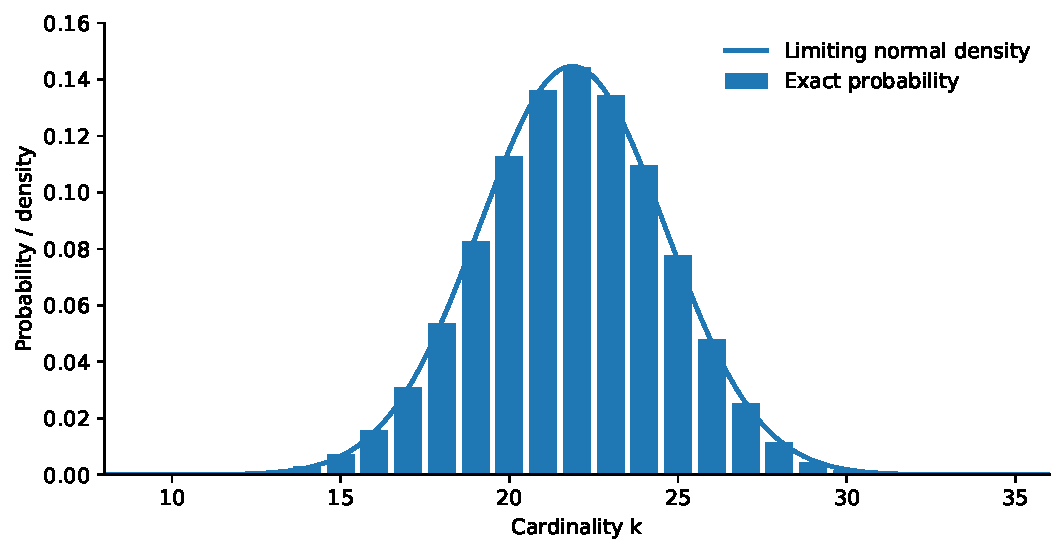
\includegraphics[width=0.92\linewidth]{figures/cardinality_distribution.pdf}
\caption{Exact cardinality probabilities for $n=20$ ($N=59$), calculated from
 $V_{20}(y)$, with the normal density using the limiting mean and variance
 from \cref{thm:clt}. The line is an illustration, not an additional claim
 of a local central limit theorem or an error bound at this finite $n$.}
\label{fig:distribution}
\end{figure}

\section{Exact algorithms and reproducibility}
\label{sec:algorithms}

\subsection{Linear-time recognition}

A direct implementation of the visibility definition examines many pairs
and shortest paths. For this graph family, \cref{lem:unique} gives a much
smaller recognizer. Given $n\ge2$ and a membership word of length $N$:
choose a zero $z$, set $b_z=0$, and visit the remaining residues by adding
three modulo $N$. At each visited position $t$, compute
$b_t=w_t(w_{t-1}\lor b_{t-3})$. Finally reject exactly when some
$b_tw_{t+1}=1$. The all-ones word is rejected separately, and every word is
accepted for $n=1$.

There are $N$ flag computations and $N$ final checks. This is $O(N)$ Boolean
work and $O(N)$ auxiliary bits in the straightforward implementation. It
does not construct the graph's $\Theta(N^2)$ adjacency relation. The code
validates the input length and the binary alphabet.

\subsection{Integer counting and coefficient computation}

To count all sets, repeated squaring computes $\tr M(1)^{3n-1}$ with
$O(\log n)$ multiplications of fixed-size matrices of integers. Alternatively,
\cref{eq:recurrence} generates the first $m$ terms in $O(m)$ integer
arithmetic operations with constant working storage, apart from the output.
These are arithmetic-operation bounds: the integers have $\Theta(n)$ bits,
so neither statement asserts constant-cost machine arithmetic.

The polynomial implementation propagates labeled edges, maintaining for
each initial and current state an array indexed by the number of ones.
This computes $V_n(y)$ in $O(N^2)$ additions of nonnegative integers and
$O(N)$ stored coefficients. It is independent of the rational coefficients
appearing in \cref{eq:binomial}. The supplied second implementation evaluates
that binomial formula using exact fractions and checks agreement.

\subsection{Exact uniform sampling}

A transfer matrix can do more than enumerate. Let $A=M(1)$ and precompute
$A^r$ for $0\le r\le N$. Choose a starting state $s$ with probability
\begin{equation}
 \frac{(A^N)_{ss}}{\tr A^N}.
 \label{eq:samplestart}
\end{equation}
With current state $u$ and $r+1$ edges remaining, choose a particular labeled
edge $e:u\to v$ with probability
\begin{equation}
 \frac{(A^r)_{vs}}{(A^{r+1})_{us}}.
 \label{eq:samplestep}
\end{equation}
The two $D\to B$ edges must remain separate choices. Their multiplicity is
already counted in the denominator. Emit each chosen edge's bit.

For any particular closed labeled walk, the successive completion counts
telescope. Multiplying \cref{eq:samplestart,eq:samplestep} gives probability
$1/\tr A^N$. By the anchored bijection, the emitted subset is therefore
exactly uniform over $\MV_n$. For $n=1$, simply choose both bits independently
with probability one half.

The implementation draws integer random numbers below the exact total
weight, not floating-point approximations to probabilities. Preprocessing
and each sample use $O(N)$ operations on large integers. The cached powers
occupy $O(N^2)$ bits, since a fixed-size matrix at exponent $r$ uses $O(r)$
bits per entry. Random-bit generation and integer arithmetic costs are not
hidden behind a claim of constant bit complexity.

\subsection{Independent tests actually performed}

The tests were run locally for this report. Their machine-readable output
is included in the archive. They use three different descriptions of
visibility, as well as independently evaluated algebraic consequences.

\begin{center}
\small
\begin{tabular}{@{}>{\raggedright\arraybackslash}p{0.31\linewidth}>{\raggedright\arraybackslash}p{0.28\linewidth}>{\raggedright\arraybackslash}p{0.33\linewidth}@{}}
\toprule
Check & Range & Observed result\\
\midrule
Direct common-neighbor graph predicate versus Boolean flag recognizer
& Every subset for $1\le n\le8$; 9,586,980 subsets
& No mismatches; every coefficient agrees with the transfer enumerator.\\[4pt]
Shortest-path BFS definition versus flag recognizer
& Every subset for $1\le n\le5$; 18,724 subsets
& No mismatches; no diameter-two assumption used by the BFS predicate.\\[4pt]
Actual labeled closed walks versus accepted membership masks
& Lengths $3n-1$, $1\le n\le5$
& Every expected mask appears exactly once; only the stated $n=1$ full-set exception.\\[4pt]
Recurrence versus integer matrix powers
& $1\le n\le250$
& Exact agreement; first 15 terms also match OEIS.\\[4pt]
Binomial formula versus polynomial dynamic programming
& $2\le n\le40$
& All coefficients agree exactly.\\[4pt]
Fixed-deficit formula versus polynomial coefficients
& $2\le n\le40$, $0\le h\le\min(9,2n-2)$
& Exact agreement.\\[4pt]
Symbolic matrix and rational identities
& Characteristic polynomial, resolvent numerator and denominator, variance formula
& Exact polynomial/rational identities verified with SymPy.\\[4pt]
Uniform sampler validity smoke test
& 7,000 words across $n=1,2,3,5,8,20,50$
& Every sampled word passes recognition. Uniformity follows from the telescoping proof, not this test.\\
\bottomrule
\end{tabular}
\end{center}

The C++ checker constructs adjacency directly from \cref{eq:graph}.
For each nonedge $\{u,v\}$ it forms
$\{u,v\}\cup(\Ngraph(u)\cap\Ngraph(v))$ and tests whether that obstruction
is contained in the subset. Separately, it constructs the cyclic pattern
obstructions and checks equality of the two families. It then compares the
graph predicate against the flag recognizer for \emph{every} subset.

The independent Python BFS check is closer still to the original definition.
For a selected source, it allows a search to reach another selected vertex
but forbids expanding that vertex. A target is visible precisely when its
restricted distance equals its distance in the original graph. Thus it does
not invoke the common-neighbor lemma or use the transfer matrix to decide
visibility.

The symbolic checker verifies the adjugate identity used in
\cref{thm:bivariate}, not merely the first several coefficients of a guessed
series. It also derives the fixed-deficit polynomials by finite symbolic
sums. None of these checks substitutes for the all-$n$ combinatorial proof.

\subsection{Files and execution}

The main executable module uses only the Python 3.9 or later standard
library. SymPy is needed only for the symbolic certificate, and Matplotlib
only to regenerate the distribution figure. A C++17 compiler is needed for
the larger exhaustive comparison. From the extracted directory, the central
commands are:
\begin{verbatim}
python code/verify.py
python code/symbolic_certificate.py
python code/visibility.py --n 20 --sample
python code/visibility.py --write-data data

g++ -O3 -std=c++17 code/exhaustive.cpp -o exhaustive
./exhaustive 8 > data/exhaustive.json
python code/verify.py

pdflatex -interaction=nonstopmode -halt-on-error article.tex
pdflatex -interaction=nonstopmode -halt-on-error article.tex
\end{verbatim}

The README gives the corresponding workflow and explains the outputs.
A SHA-256 manifest covers the deliverable files. No compiler binary, virtual
environment, font file, or fetched third-party paper is required in the ZIP.

\section{What the argument establishes, and what it does not}
\label{sec:scope}

The selected conjecture is resolved by a bijection, followed by a finite
matrix calculation. Its rational denominator is the characteristic data of
$M(y)^3$, because the graph order advances by three when $n$ increases by
one. The nonproper numerator records the genuine exceptional first graph;
it is not a numerical nuisance to be suppressed.

The strongest structural refinement is that the entire cardinality
polynomial comes from the same four-state system. The return-block
decomposition then gives a finite formula for every coefficient, exact
maximum-set classification, and an infinite family of eventual polynomial
formulas indexed by the deficit $h$. Perron theory controls typical sets,
while the defect identity controls the extreme tail.

Several matters are deliberately left outside the claims. We do not assert
that the four-state presentation is the unique or minimal deterministic
presentation of the underlying binary language. The minimality statement
proved above concerns the scalar eventual recurrence, not automata. We do
not claim that the size polynomials have real zeros or any unproved global
log-concavity property. A central limit theorem is proved, but no local limit
theorem or finite-$n$ normal-approximation error is asserted. Finally, the
literature search documents a conjecture that remained labeled open in the
consulted source; it does not establish exclusive priority for every
corollary derived here.

The method suggests concrete further investigations without requiring any
of them for the present result: enumeration modulo graph automorphisms,
additional vertex weights, and related circulant families whose
common-neighbor obstructions admit finite-state compression. Such extensions
must check periodic-state multiplicities anew. The coprimality and zero-reset
arguments in this proof are precisely the features that should not be
silently assumed to survive a change of graph family.

\appendix
\section{Sequence values and coefficient data}
\label{app:data}

The first fifteen entries below agree with the values displayed by OEIS on
the consultation date \cite{oeis}. The remaining displayed entries and the
extended file are calculated from the proved recurrence and independently
checked by matrix powers.
\begin{center}
\begin{tabular}{@{}rr@{\qquad}rr@{}}
\toprule
$n$ & $a_n$ & $n$ & $a_n$\\
\midrule
1 & 4 & 11 & 213,940,607 \\
2 & 21 & 12 & 1,291,991,757 \\
3 & 127 & 13 & 7,802,356,615 \\
4 & 749 & 14 & 47,118,492,485 \\
5 & 4,455 & 15 & 284,548,794,383 \\
6 & 26,725 & 16 & 1,718,391,139,389 \\
7 & 161,007 & 17 & 10,377,369,263,383 \\
8 & 971,613 & 18 & 62,668,963,071,925 \\
9 & 5,866,487 & 19 & 378,458,048,186,527 \\
10 & 35,426,517 & 20 & 2,285,509,240,092,589 \\
\bottomrule
\end{tabular}
\end{center}

For illustration, the next two size polynomials after those in
\cref{sec:gf} are
\begin{align*}
V_6(y)={}&1+17y+136y^2+663y^3+2142y^4+4692y^5\\
 &+6885y^6+6579y^7+3944y^8+1394y^9+255y^{10}+17y^{11},\\
V_7(y)={}&1+20y+190y^2+1120y^3+4505y^4+12844y^5\\
 &+26190y^6+37820y^7+37910y^8+25680y^9\\
 &+11292y^{10}+3000y^{11}+415y^{12}+20y^{13}.
\end{align*}
The file \texttt{data/visibility\_coefficients.csv} has columns
\texttt{n, vertices, cardinality, count}. It records nonzero coefficient
ranges, including the constant coefficient, through $n=50$.
The file \texttt{data/b391632\_extended.txt} has 250 indexed terms in
b-file-style format. These are locally derived data; the file is not
represented as an official OEIS submission.

\section{A dependency map for auditing the proof}
\label{app:audit}

The logical dependencies can be audited without running any code:
\begin{enumerate}
\item The circulant definition gives the exact common-neighbor set in
\cref{lem:neighbors}. This step is where graph geometry enters.
\item A selected nonedge is blocked precisely by selecting all common
neighbors, giving \cref{eq:forbidden}. The periodic-extension lemma removes
the graph-dependent upper bound on pattern length.
\item The flags remember every possible finite prefix by
\cref{eq:flag}. The zero-reset argument and $\gcd(3,3n-1)=1$ prove that
periodic flags cannot introduce spurious multiplicity or unsupported states.
\item The six semantic states exhaust the valid possibilities. The explicit
incoming-edge lift proves that their four-state quotient preserves closed
labeled walks.
\item The anchored bijection justifies the trace identity. Everything
thereafter follows from matrix algebra, first-return blocks, or the
Perron eigenvalue.
\end{enumerate}

The main edge cases are the empty word, the all-ones word, the full subset
of $G_1$, patterns crossing vertex $0$, patterns longer than one period,
and repeated cyclic words. Each is handled explicitly in
\cref{sec:patterns,sec:automaton}. The fixed-deficit theorem excludes the
empty-set target by its stated eventual range; no zero-cardinality term
has been inadvertently included in its block sum.

\begin{thebibliography}{9}
\bibitem{oeis}
E. W. Weisstein and A. Howroyd,
\emph{A391632: Number of mutual-visibility sets in the $n$-Andr\'asfai graph},
The On-Line Encyclopedia of Integer Sequences.
Entry created 14 December 2025; generating function conjectured by
A. Howroyd, 12 January 2026; consulted 19 September 2026.
\url{https://oeis.org/A391632}.

\bibitem{distefano}
G. Di Stefano,
\emph{Mutual Visibility in Graphs},
arXiv:2105.02722, version 2, 15 July 2021.
\url{https://arxiv.org/abs/2105.02722}.

\bibitem{metric}
A. Behtoei, S. Payrovi, and S. B. Pejman,
\emph{Metric dimension of Andrasfai graphs},
arXiv:1706.06852, 21 June 2017.
The circulant definition is in the introduction.
\url{https://arxiv.org/abs/1706.06852}.
\end{thebibliography}
\end{document}
